%% Requires compilation with XeLaTeX or LuaLaTeX
%% based on UC Berkeley Beamer theme https://www.overleaf.com/latex/templates/uc-berkeley-beamer-theme/bywswngntrws
\documentclass[10pt,xcolor={table,dvipsnames},t]{beamer}

\usetheme{UCBerkeley}
\setbeamertemplate{footline}[frame number] 
\RequirePackage[style=numeric]{biblatex}
\addbibresource{refs.bib}
\RequirePackage{csquotes}
\RequirePackage{amsmath}
\RequirePackage{physics}
\RequirePackage{graphicx}
\RequirePackage[font=small]{caption, subcaption}
\RequirePackage{wrapfig}
\RequirePackage{siunitx}
\RequirePackage{sidecap}
\RequirePackage{caption}
\captionsetup[figure]{font = scriptsize, labelfont = scriptsize} % https://tex.stackexchange.com/questions/52132/beamer-change-size-of-figure-caption
\setkeys{Gin}{width=1\linewidth}


\title[Autosailboat]{Autonomous control of a sailboat}
\author{Neelay Junnarkar, Andrew Fearing, Hamza Khawaja}
% \institute{Your Faculty/Department}
\date{\today}

\begin{document}

\begin{frame}
  \titlepage
\end{frame}

\begin{frame}{Outline}
 \tableofcontents
\end{frame}
\section{Introduction}
\begin{frame}{Team}

Neelay Junnarkar

\hfill\\
Andrew Fearing

\hfill\\
Hamza Khawaja
\end{frame}


\begin{frame}{Motivation}
\begin{columns}
\column{0.5\linewidth}
    \begin{figure}
        \centering
        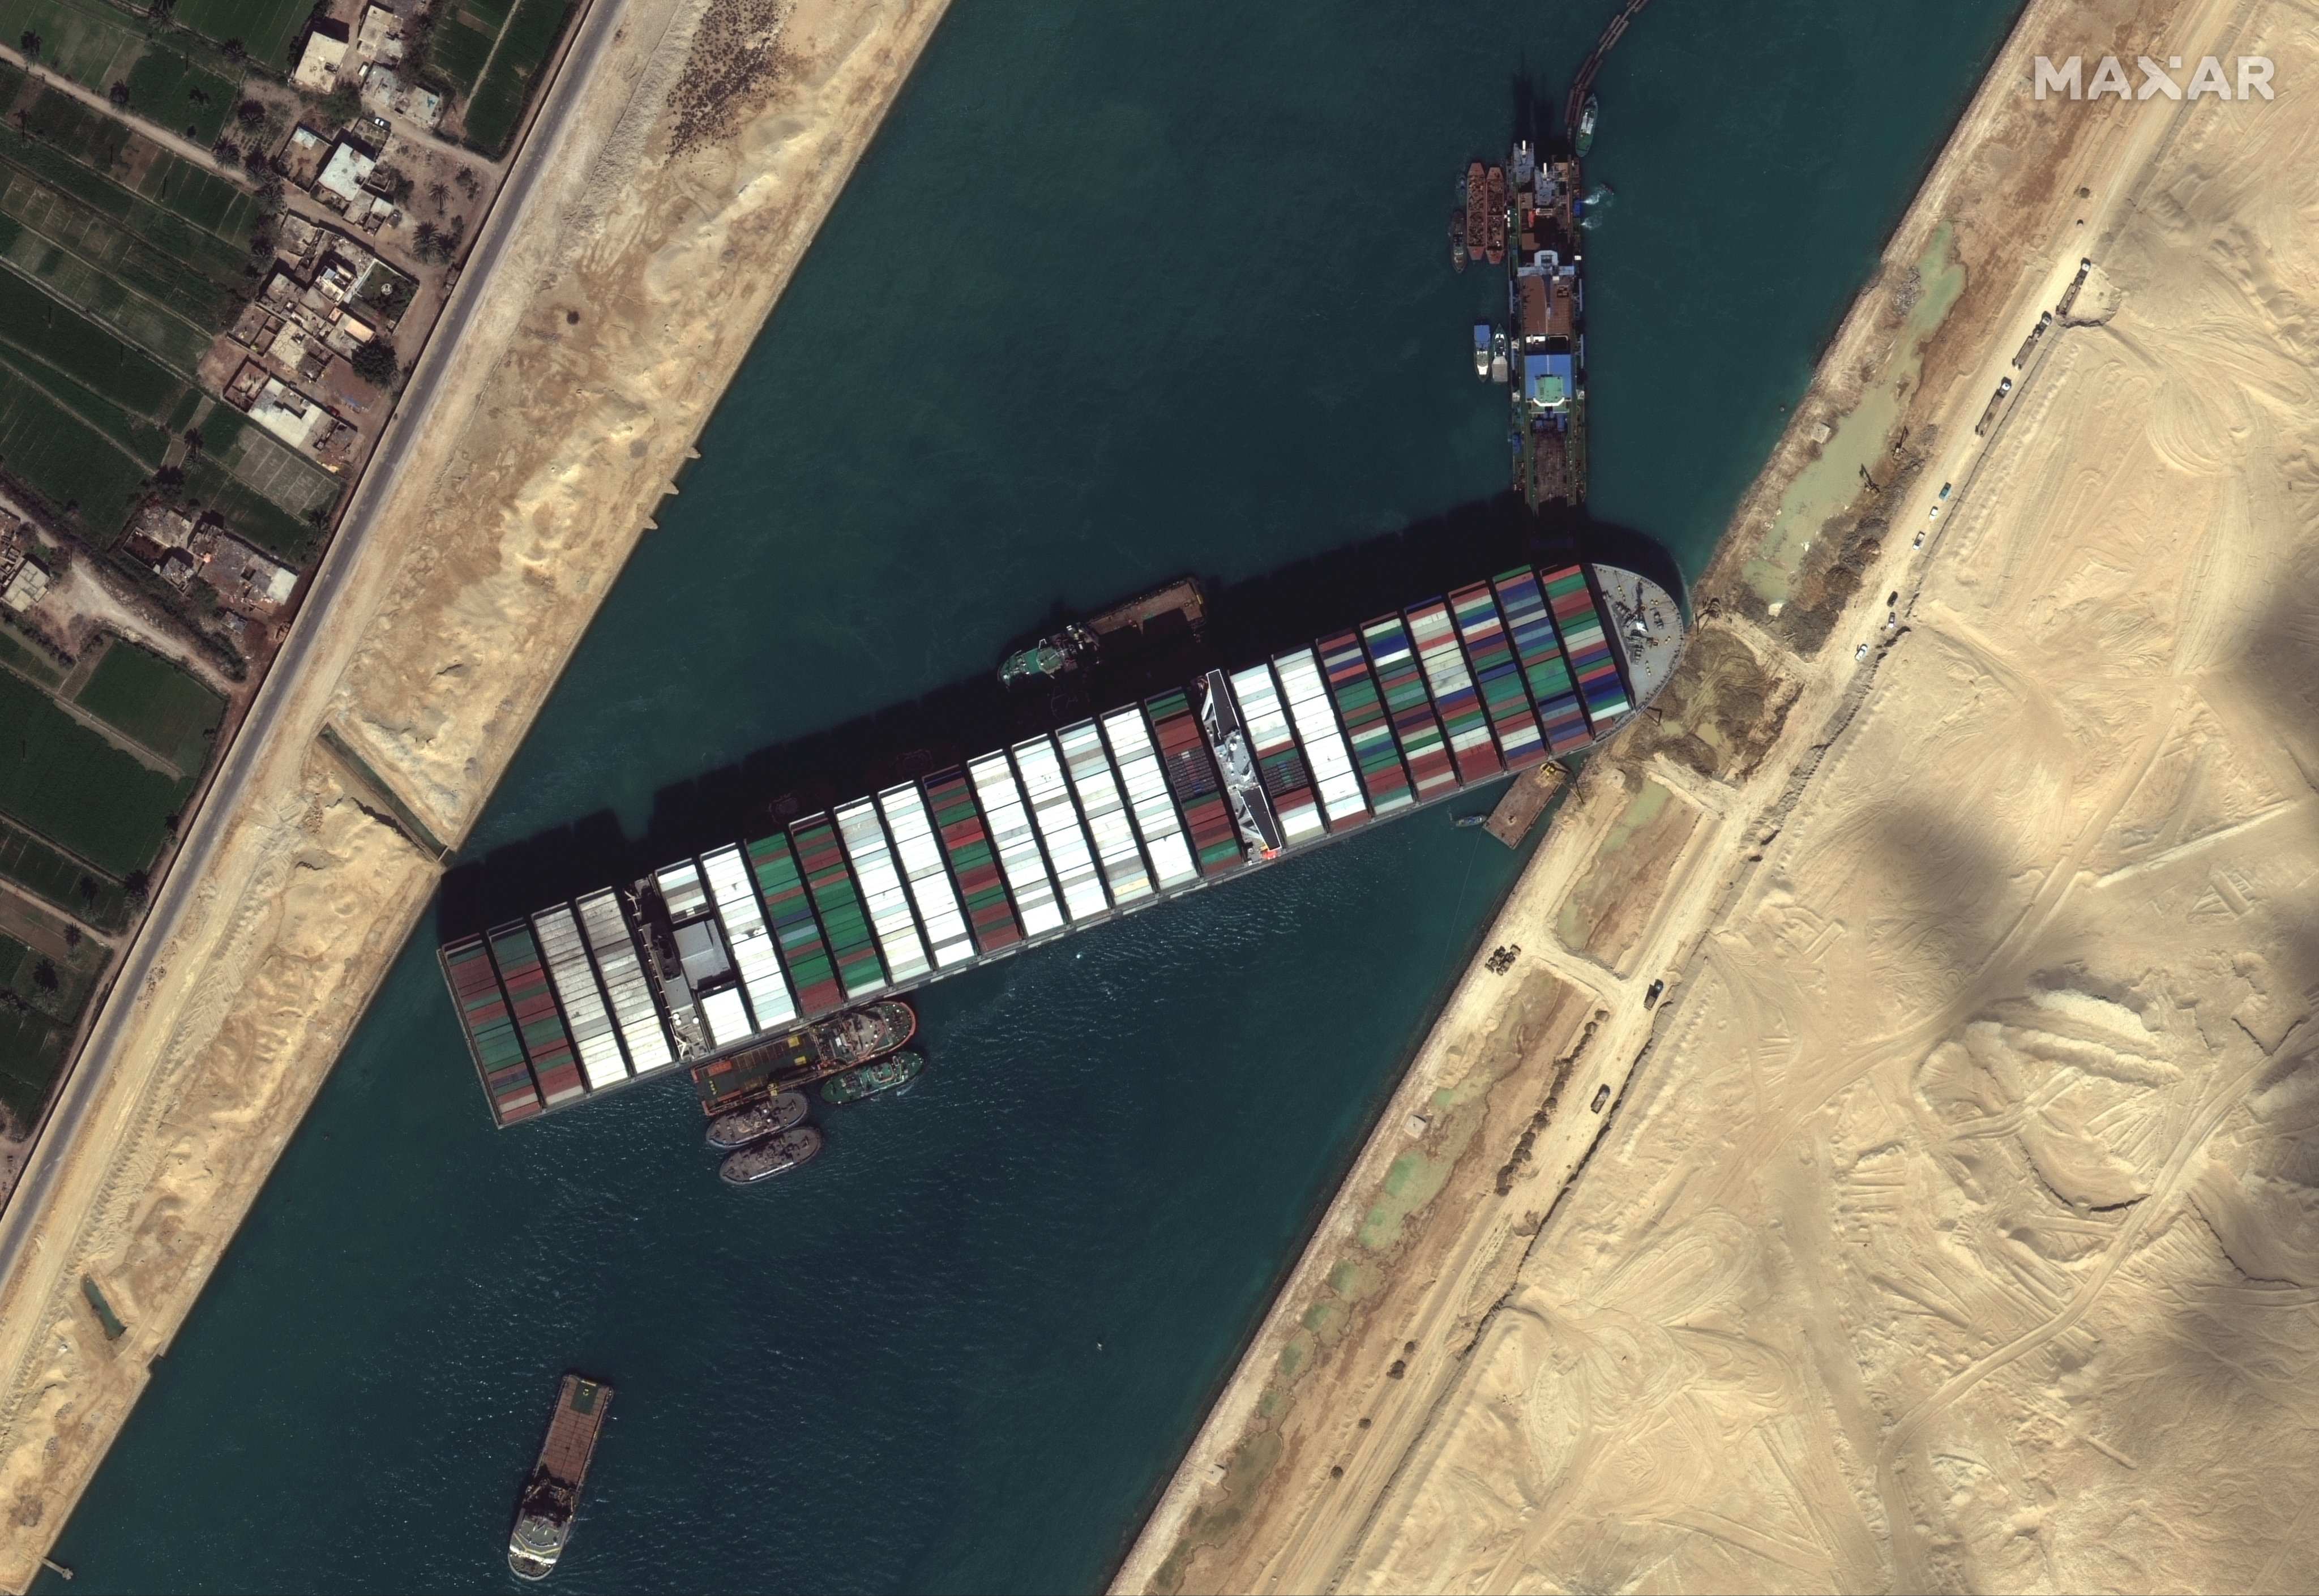
\includegraphics{documents/figures/Suez_Canal_blocked_by_Ever_Given_March_27_2021.jpg}
        \caption{Boat stuck}
        \label{fig:boat_stuck}
    \end{figure}  
\column{0.5\linewidth}
    \textbf{Control of sailboats}
    
    \hfill\\
    Controlling boats autonomously presents an interesting challenge due to the out-sized effect of environmental disturbances such as wind, water currents, and waves. 
    
    \hfill\\
    \textbf{Why Sailboats?}
    
    \hfill\\
    Sailboats are useful for low-power long-term deployments.
    
\end{columns}
\end{frame}

\begin{frame}{Goal}

\begin{enumerate}
    \item Develop sailboat yaw controller.
    \item Develop path planner which can navigate channels.
\end{enumerate}
Focus on robustness to environmental disturbances.

\end{frame}
  

\begin{frame}{Sailboats}
\begin{columns}
\column{0.4\linewidth}
\begin{figure}
    \centering
    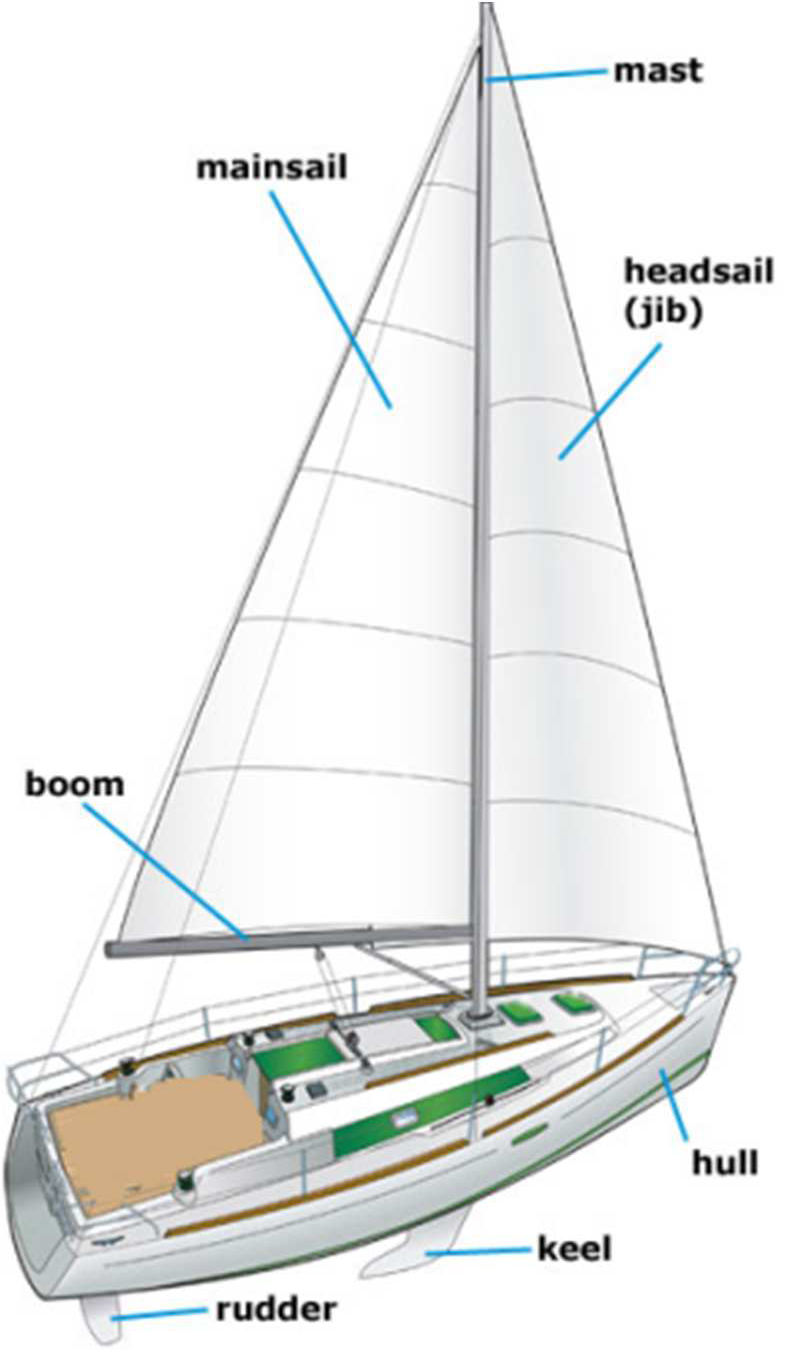
\includegraphics[width=0.3\linewidth]{documents/figures/alves_sailboat.png}
    \caption{Alves sailboat \cite{Alves2010}}
    \label{fig:alves_sailboat}
\end{figure}

\begin{figure}
    \centering
    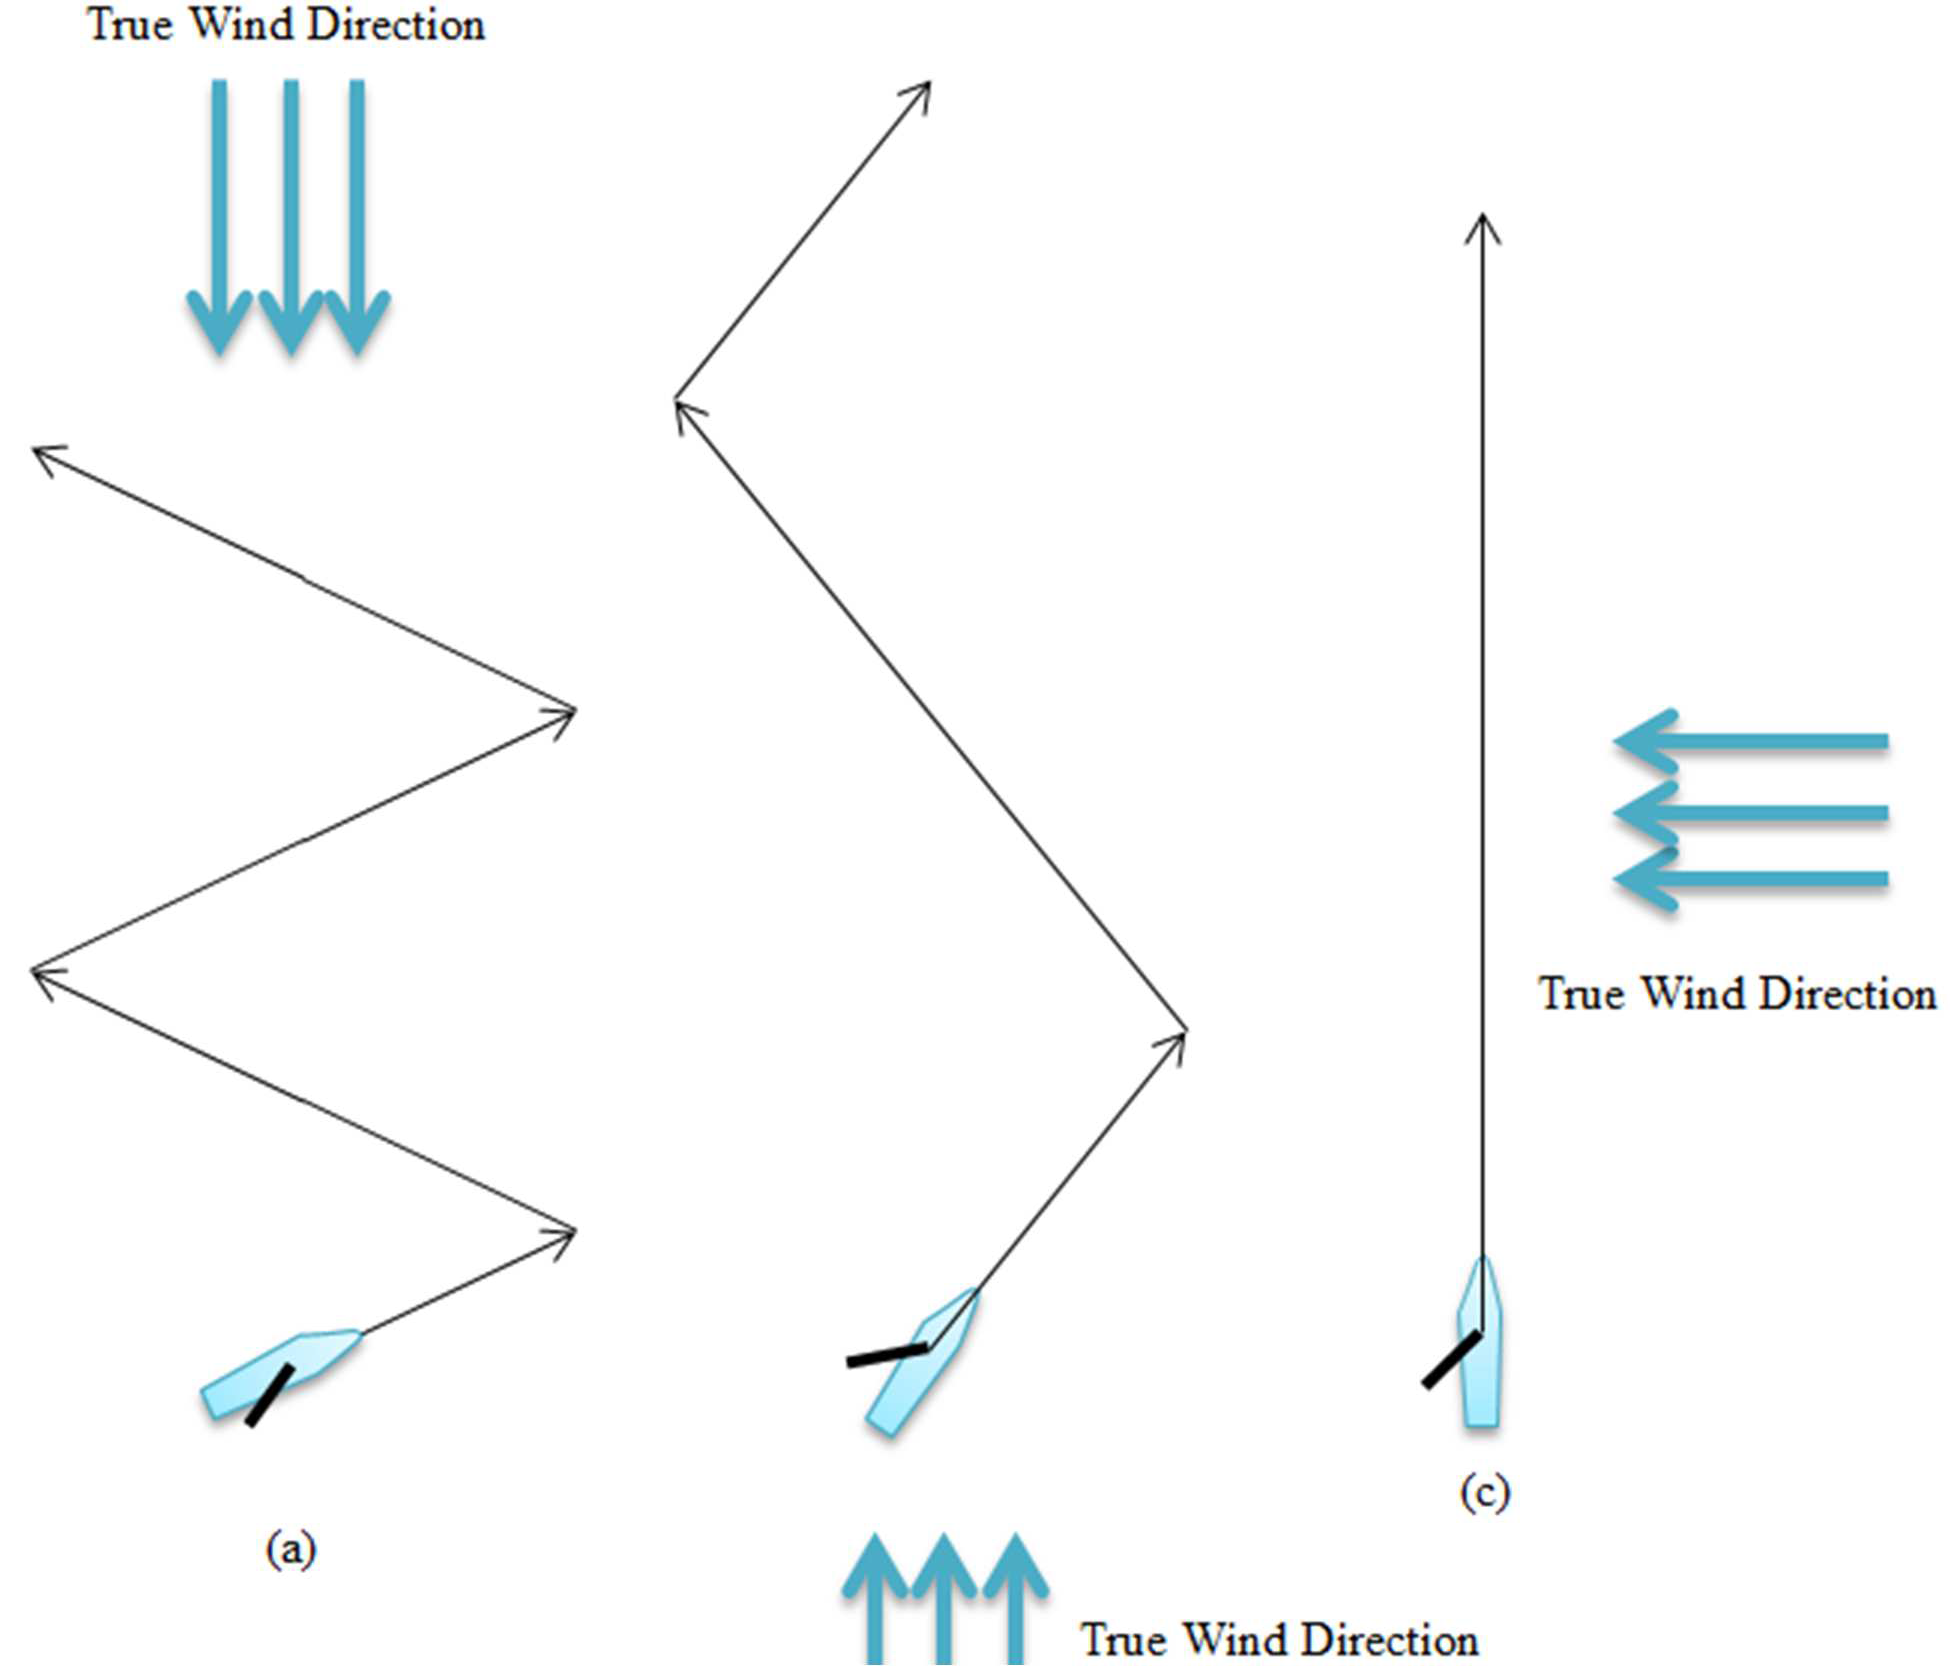
\includegraphics[width=0.75\linewidth]{documents/figures/alves_modes.png}
    \caption{Modes of sailing \cite{Alves2010}}
    \label{fig:alves_modes}
\end{figure}
\column{0.4\linewidth}
\begin{figure}
    \centering
    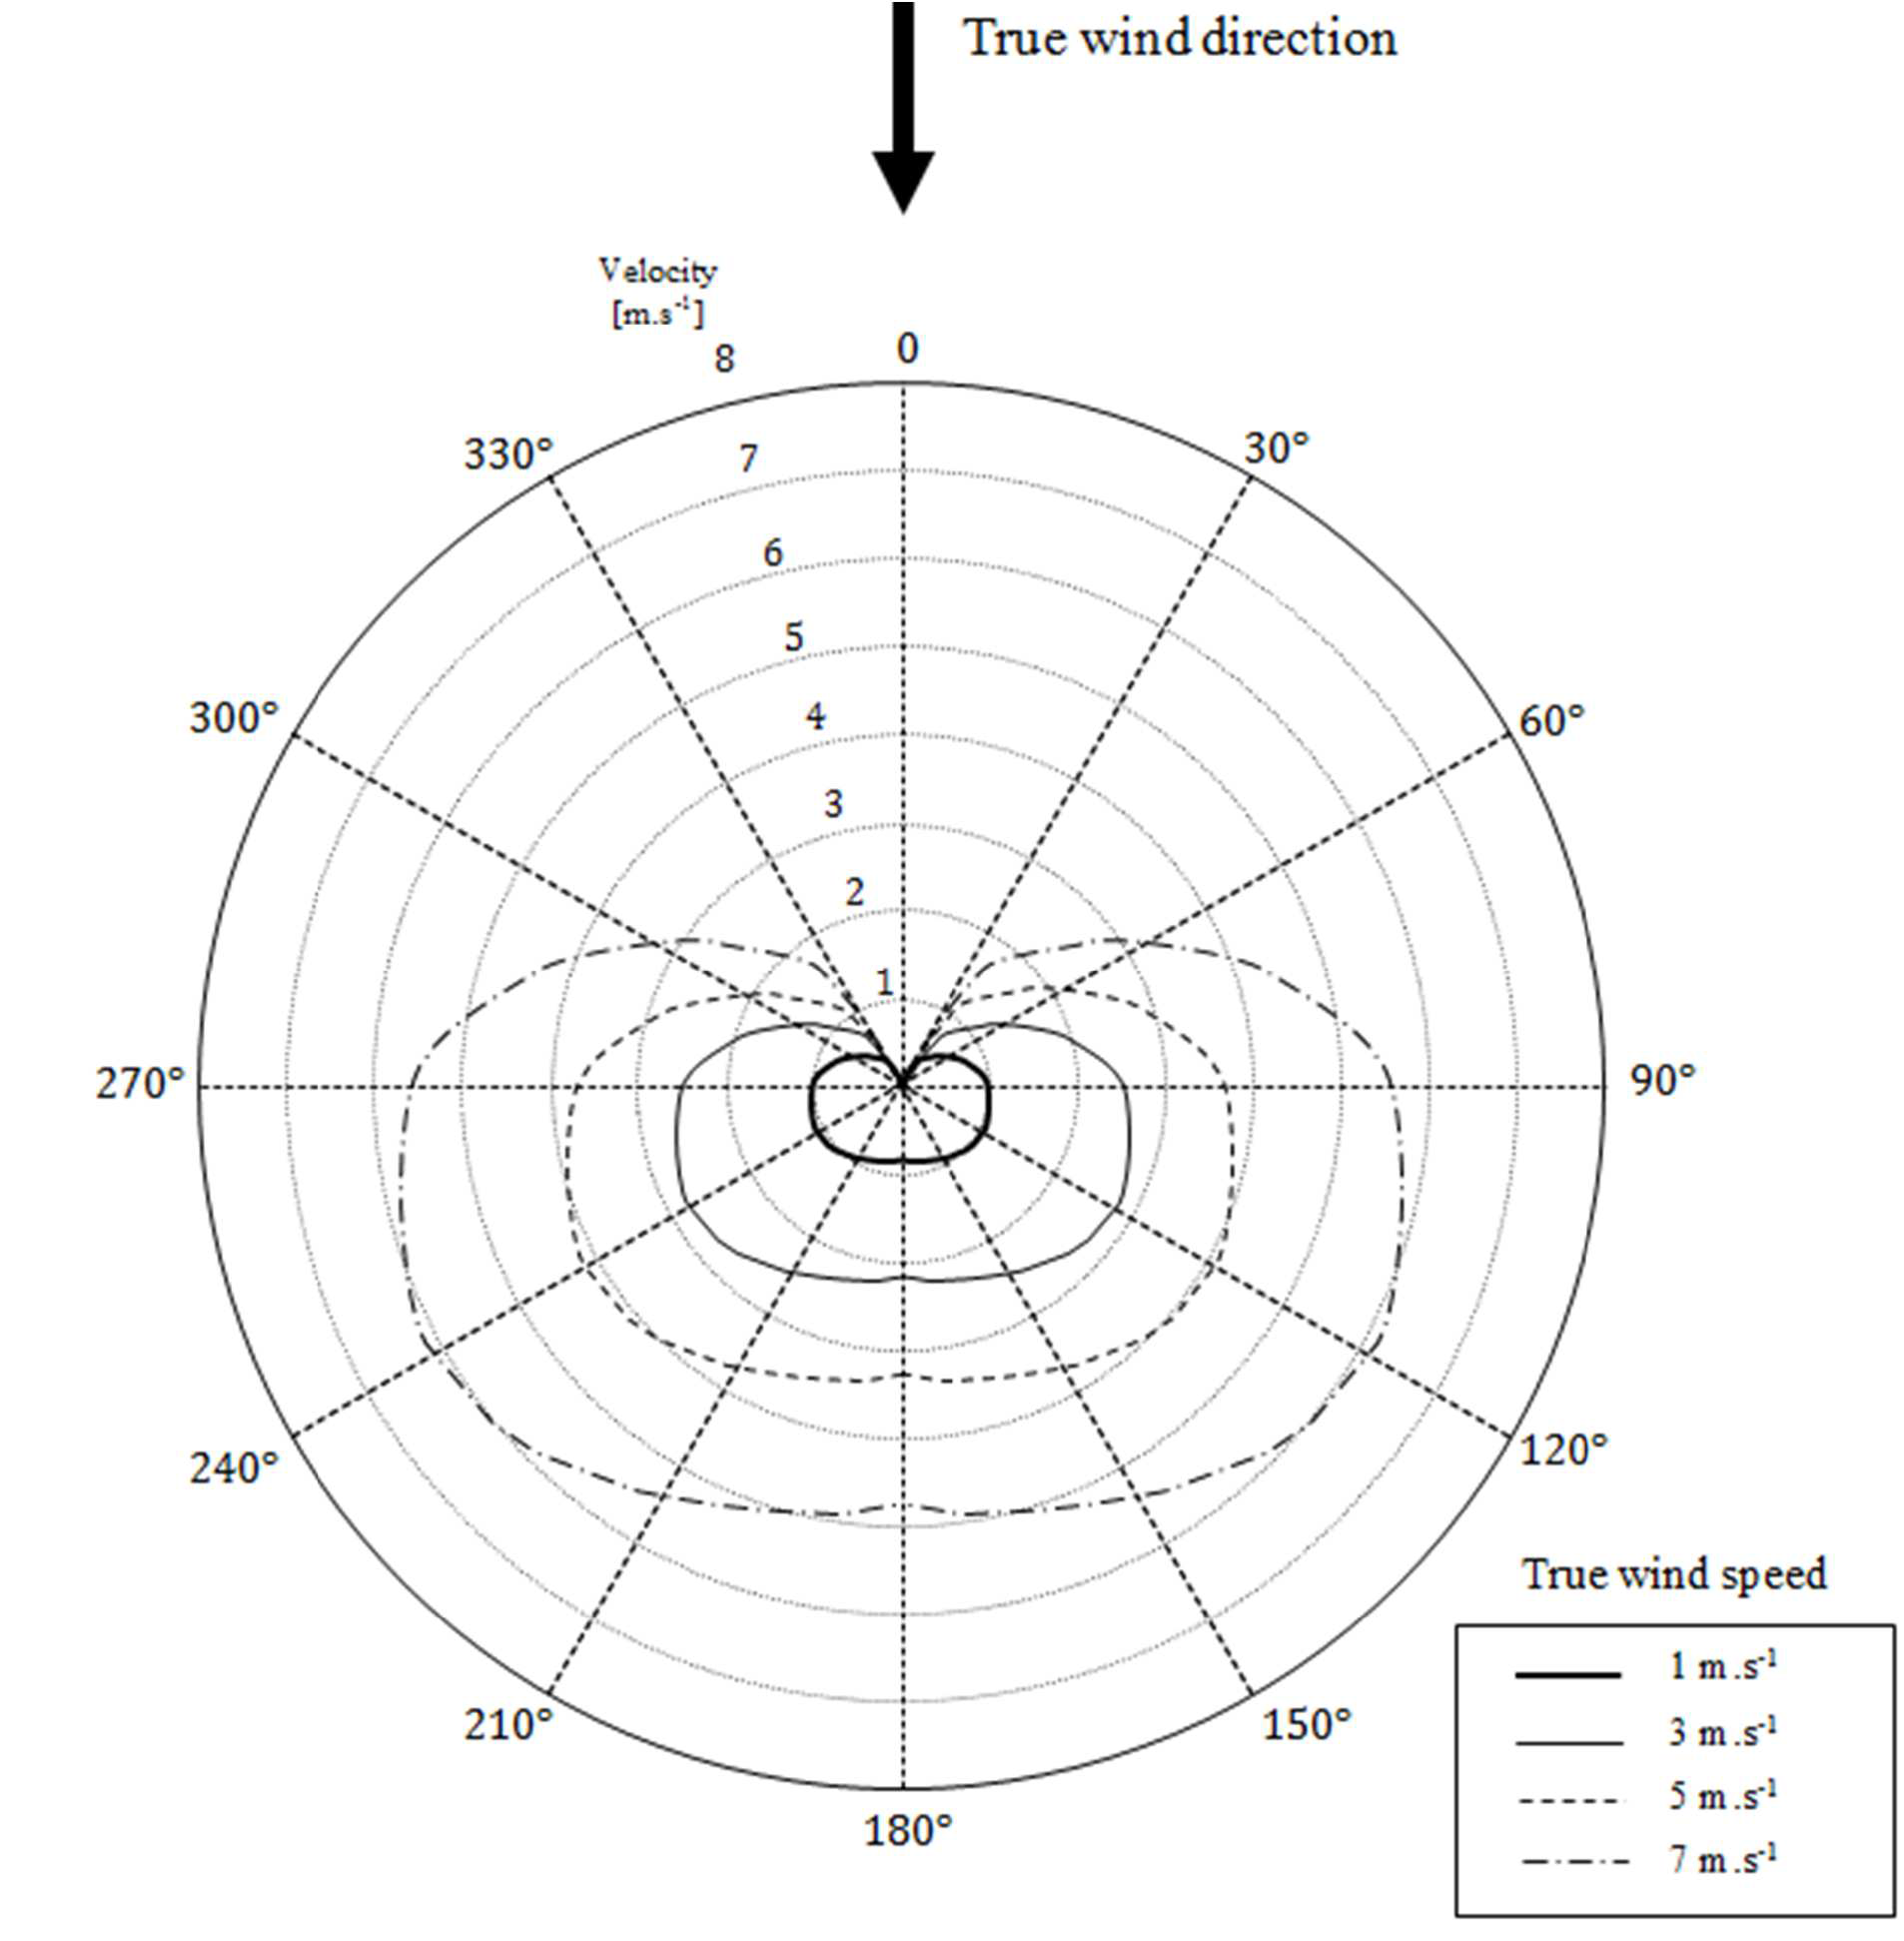
\includegraphics[width=0.7\linewidth]{documents/figures/alves_vpp.png}
    \caption{Velocity polar diagram \cite{Alves2010}}
    \label{fig:alves_velocity}
\end{figure}
\end{columns}
\end{frame}

\section{Progress}
\begin{frame}{What we've done}
    
    
        Evaluated two different simulators for unmanned surface vehicles
    \begin{columns}
    \column{0.5\linewidth}
        USVSim \cite{Paravisi2019}
        \begin{itemize}
            \item Ubuntu 16.04 + Kinetic ROS + Gazebo
            \item 6 DoF
            \item Waves, buoyancy, water currents, wind currents, thruster underwater, thruster above water, foil
            \item Too complicated, hard to extend
        \end{itemize}
    \column{0.5\linewidth}
        stda-sailboat-sim \cite{Buehler2018}
        \begin{itemize}
            \item Python + Numpy + Matplotlib
            \item 6 DoF
            \item sail, keel, rudder force. Buoyancy force, wave resistance, damping forces.
            \item Good enough
        \end{itemize}
    \end{columns}
\end{frame}
\begin{frame}{What's working so far}
\begin{columns}
\column{0.5\linewidth}
    \begin{figure}
        \centering
        \begin{subfigure}
            \centering
            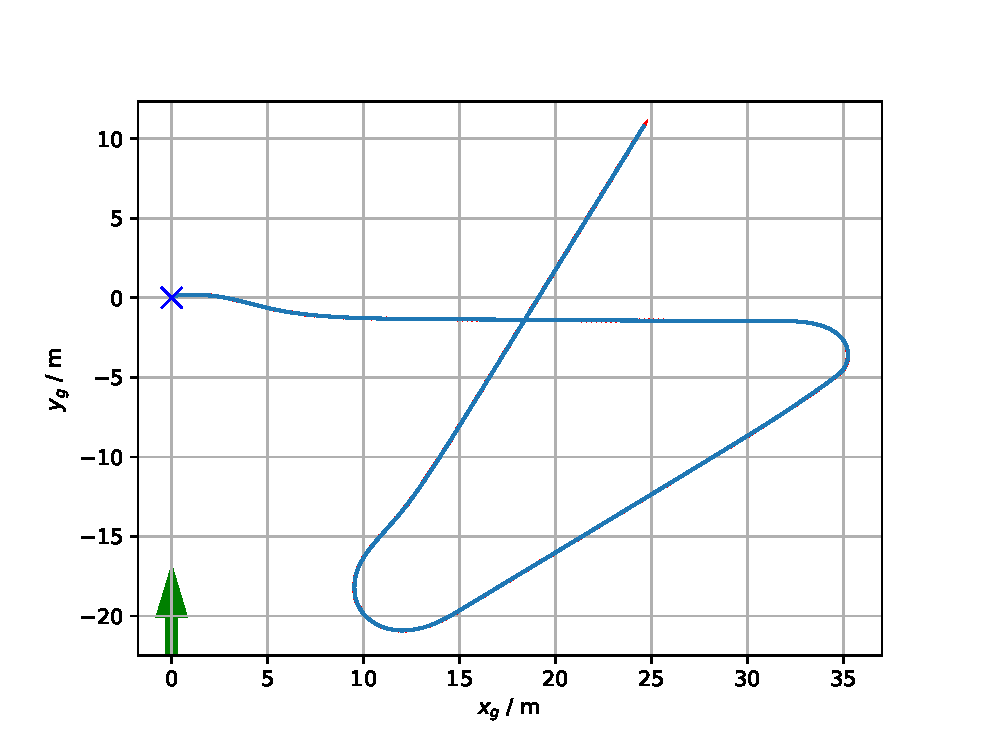
\includegraphics{documents/figures/trajectories.eps}
            \caption{Caption}
            \label{fig:my_label}
        \end{subfigure}
        \begin{subfigure}
            \centering
            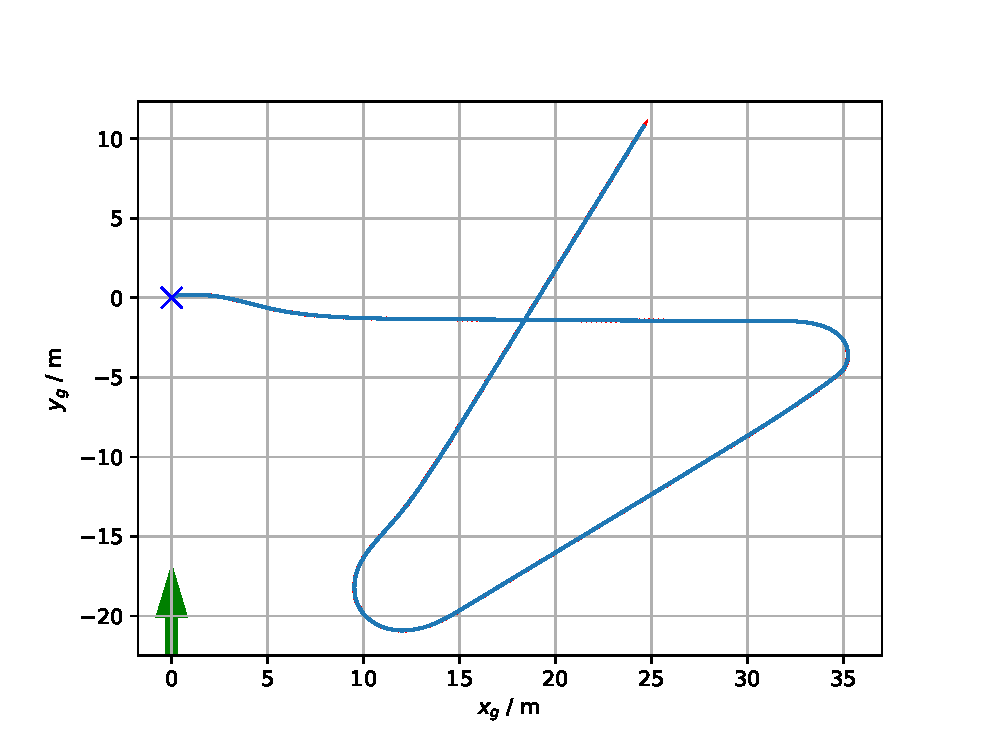
\includegraphics{documents/figures/trajectories.eps}
            \caption{Caption}
            \label{fig:my_label}
        \end{subfigure}
    \end{figure}
\end{columns}

\end{frame}


\section{Future work}

\begin{frame}{The game plan}

\end{frame}
\begin{frame}{Roadblocks}
    
\end{frame}
\begin{frame}{References}
    \printbibliography{}
\end{frame}

\end{document}